\question 对于下列关键字序列,不可能构成某二叉排序树中一条查找路径的序列是( )
\par\fourch{\textcolor{red}{95,22,91,24,94,71}}{92,20,91,34,88,35}{21,89,77,29,36,38}{12,25,71,68,33,34}
\begin{solution}各选项的查找过程如下图所示,从中看到,选项A对应的查找树中在91的左子树中出现了大于91的94(即为图中虚线圈内部分),因此A选项不可能。
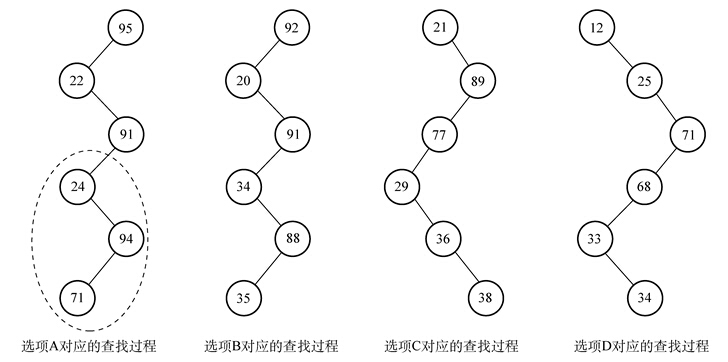
\includegraphics[width=7.58333in,height=3.77083in]{computerassets/0541e42c6cfafd6de4847b09c02eae6e.jpeg}
【总结】
本题属于比较基础的题目。根据二叉排序树的性质即可求解。二叉排序树或者是空树,或者是满足以下性质的二叉树:
① 若左子树非空,则左子树上所有记录值小于根记录的值。 ②
若右子树非空,则右子树上所有记录值大于根记录的值。 ③
左、右子树本身各是一棵二叉树。
\end{solution}
\question (江苏大学,2004年)对二叉排序树进行(
)遍历,可以得到该二叉树所有节点构成的排序序列
\par\twoch{前序}{\textcolor{red}{中序}}{后序}{层次}
\begin{solution}考察二叉排序的树的特征以及二叉树的中序遍历,只有中序遍历才是按照节点的关键字的大小递增排序
\end{solution}
\question (南京林业大学,2005年)不满足平衡查找树概念的是( )
\par\twoch{\textcolor{red}{BST树}}{AVL树}{折半查找判定树}{B+树}
\begin{solution}二叉查找树(BST)不一定是平衡的
\end{solution}
\question (青岛大学,2004年)为了采用动态查找表进行高效的查找,数据的组织结构最好采用(
)
\par\twoch{有序表}{线性链表}{\textcolor{red}{二叉排序树}}{分块有序表}
\begin{solution}四个选项中,二叉排序树的查找效率最高,有序表不支持动态,链表查找不高效
\end{solution}
\question (北京交通大学,2004年)在含有n个节点的二叉排序树中查找一个关键字,进行关键字比较次数最大值是(
)
\par\twoch{n/2}{logn}{log(n+1)}{\textcolor{red}{n}}
\begin{solution}看到这题,很多人可能很快地选择B,认为一棵树的高度为logn,进行关键字较次数最大应当是这棵树的高度;其实不然,这是因为没有考虑到特例的情况,因为既然是题目中要求比较次数的最大值,那么特殊情况就是如果这棵树就是n层,每层1个节点的话,此时它的高度最高为n,则进行关键字比较次数最大值为n
\end{solution}
\question (中国科学技术大学,2004年)分别以下列序列构造二叉排序树,与众不同的的是(
)
\par\fourch{\textcolor{red}{100,80,60,85,110,120,150}}{100,80,60,85,120,110,150}{100,80,85,60,120,110,150}{100,80,60,85,120,150,110}
\begin{solution}各序列对应的二叉排序树如图所示:
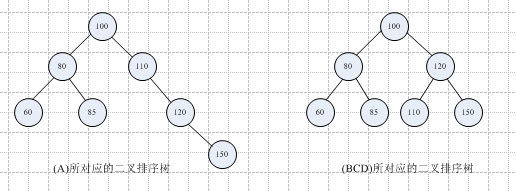
\includegraphics[width=5.37500in,height=1.98958in]{computerassets/e35aeff3fcf8b84414a7eac48edcb852.png}
\end{solution}
\question (南京邮电大学,2005年)已知一棵由关键字集合\{18,43,27,77,44,36,39\}所构造的二叉搜索树,对该树进行中序遍历得到的节点序列为(
)
\par\twoch{树形未定,无法确定}{18,43,27,77,44,36,39}{\textcolor{red}{18,27,36,39,43,44,77}}{77,44,43,39,36,27,18}
\begin{solution}对二叉搜索树进行中序遍历的结果一定是一个从小到大的有序序列
\end{solution}
\question (南京邮电大学,2006年)在一棵二叉搜索树上搜索一个元素的平均时间复杂度是(
)
\par\fourch{}{O(n)}{O(nlogn)}{\textcolor{red}{O(logn)}}
\begin{solution}考察二叉搜索树的概念,平均情况下时间复杂度为O(logn)
\end{solution}
\question (北京交通大学,2005年)设二叉排序树中关键字由1到1000的整数构成,现要查找关键字为363的节点,下述关键字序列中,不可能是在二叉排序树上查找的序列是(
)
\par\fourch{2,252,401,398,330,344,397,363}{924,220,911,244,898,258,362,363}{\textcolor{red}{925,202,911,240,912,245,363}}{2,399,387,219,266,382,381,278,363}
\begin{solution}C选项中的关键字911节点,比较目标关键字363,363应该位于911的左子树中,故根据二叉排序树的性质,911后面的关键字都应该位于其左子树中,从而均应该比911小,关键字912与性质矛盾
\end{solution}
\question (华南理工大学,2005年)利用逐点插入法建立序列(60,74,44,99,75,30,36,45,68,9)对应的二叉排序树以后,查找元素75要进行(
)次元素间的比较
\par\twoch{\textcolor{red}{4}}{3}{7}{5}
\begin{solution}逐点插入法建立的二叉排序树如图所示,所以分别需要跟60,74,99,75进行比较
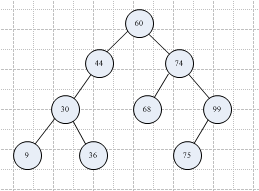
\includegraphics[width=2.69792in,height=1.98958in]{computerassets/a660a0e92897a903a7842a30c0b2bfee.png}
\end{solution}
